
\documentclass{standalone}

\usepackage{tikz}

\begin{document}

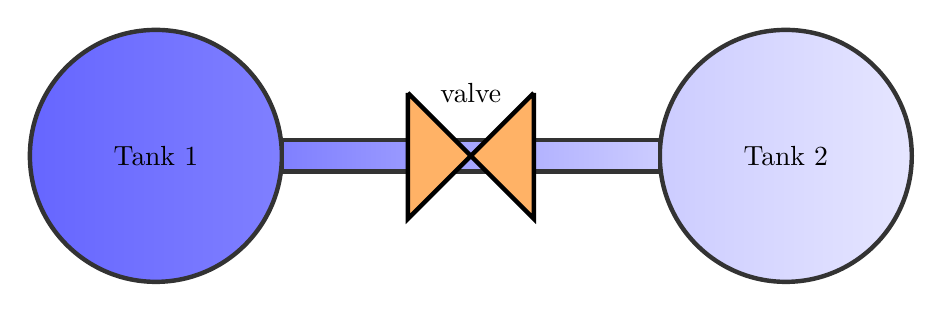
\begin{tikzpicture}[thick, scale=0.8]
  \filldraw [black!80, left color=blue!60, right color=blue!50, ultra thick] (2,2)circle [radius = 2];
  \filldraw [black!80, left color=blue!20, right color=blue!10,, ultra thick] (12,2)circle [radius = 2];
  \filldraw [black!80, left color=blue!50, right color=blue!20, ultra thick] (4,1.75) rectangle (10,2.25);
  \draw [black, fill=orange!60, ultra thick] (6,3) -- (7,2) -- (6,1) -- (6,3);
  \draw [black, fill=orange!60, ultra thick] (8,3) -- (7,2) -- (8,1) -- (8,3);
  \node at (7,3) {valve};
  \node at (2,2) {Tank 1};
  \node at (12,2) {Tank 2};
\end{tikzpicture}

\end{document}